
In this chapter we will review the main concepts and theory needed to understand the rest of this thesis.
We will start with a brief introduction of the Dynamical Systems (DS) theory and an overview of Machine Learning
concepts and foundational models that will be useful to understand the rest of the work.
%Then we will move to a more specific topic, about RC and the ESN model, 
%with some enphasis on the Deep counterparts of both models treated in this work.


\section{The Inherent Dynamism of Natural Systems}\todo{questo va nel background}
Our universe is essentially a complex non-linear dynamical system, and since Newton in mid 1600s, used differential equations as a method
to solve the two body problems, but many natural phenomena are essentially Complex Systems, from small components of the 
environment there are interdependaces \todo{devo approfondire i sistemi complessi?} (CS) which exhibit dynamics that evolve through time:
such as motion of planets, flow of fluids, weather changes, growth of population and many others phenomena.\newline

Dynamics is a fundamental piece of reality and modeling time dependent system evolution, is crucial to understand the world around us:
eg. the design of control system, stock market and also the human brain can be modeled as a dynamical system.
\todo{forse questa parte sui framework non va messa qui} The methodological framework developed through the preceding century have been specifically designed to analyze sequential data structures, commonly referred as \textit{time series},
These approaches encompass techniques such as Autoregressive (AR) 
models (i should cite but cannot find source) which employ linear regression on data sequences,
extending to more sophisticasted frameworks including State-Space Models \cite{kalman1960new}, originally developed for Control Theory applications,
 and Hidden Markov Models (HMM) \cite{baum1966statistical}. The latter served as fundational precursors to Recurrent Neural Netowrks \cite{ELMAN1990179} (RNNs).
 The aforementioned models, are the basis of modern neural based sequential modeling.\newline


\section{Dynamical Systems review}
A dynamical system is a system which evolves over time, we can describe it's changes throught \textbf{state variables}, usually many models are constructed such that
only the foundamental state variables are considered, for example \textit{biological spiking neurons} modeled as in \cite{1257420} are described by a simple 2-D dimensional ODE, where the two state variables are the membrane potential and a recovery variable.
ignoring existing other possible variables such gradient of ion concentration, temperature; for the sake of obtaining a large scale simulation.\newline

There are two types of dynamical systems: \textit{Differential Equations}, which are continuous in time,
and Difference Equations or \textit{Iterated Maps} which are discrete in time. 
The most used in a wide range of sciences fields are the former, which are further distinguished in Ordinary Differential Equations (ODE) 
and Partial Differential Equations (PDE), the difference is that in PDE we have two or more independent variables.  \newline

This thesis will focus on ODEs since our models fell into that category, but we will also use \textit{discretization methods} (link to the section maybe) to obtain it's approximated solution.\newline
 Formally we define an ODE as:
\begin{equation}
    \frac{d\mathbf{x}}{dt} = f(\mathbf{x},t)
\end{equation}
where $\mathbf{x} \in \mathbb{R}^n$ is the state vector, $t$ is the time and $f:\mathbb{R}^n \times \mathbb{R} \rightarrow \mathbb{R}^n$ is a
vector field grouping all the state variables that describe the evolution of the system. \newline

\todo{questo va tolto, forse è meglio non andare troppo in dettaglio con queste cose}
An example of ODE is the well known Dampened Harmonic Oscillator:
\begin{equation} \label{eq:armonic}
    \frac{d^2x}{dt^2} + 2\beta \frac{dx}{dt} + \omega_0^2 x = 0
\end{equation}
where $x$ is the position of the oscillator, $\beta$ is the damping coefficient and $\omega_0$ is the natural frequency of the oscillator.
\todo{anche questo va tolto?}

A Differential Equation is \textit{autonomous} if the function $f$ does not depend explicitly on time, otherwise is \textit{non-autonomous}.
We can switch from a non-autonomous to an autonomous system by adding time as a new variable to the state vector, for example the
non-autonomous system of equation \ref{eq:armonic} can be rewritten with a change of variable.

\clearpage
\subsection{Modeling}
Modeling is a central methodology in the study of complex systems, translating real world observations and hypoteses into a formalized mathematical model, even tough simplified, can be
crucial for studying emergent behaviours, particlarly in natural systems where we cannot change the initial state, or the enviroment variables that influence it.
\newline
The Hodgkin-Huxley model \cite{hodgkin1952quantitative} describes the dynamics of neuronal membrane
potential through an equivalent electrical circuit. The membrane can be represented as a capacitor $C_m$ 
in parallel with several ion channels, each modeled as a voltage-dependent conductance 
in series with a battery representing the ion's reversal potential.
\newline
\begin{figure}[H]
    \centering
    \begin{tabular}{m{0.35\textwidth}@{\hspace{1cm}}c@{\hspace{1cm}}m{0.45\textwidth}}
        \centering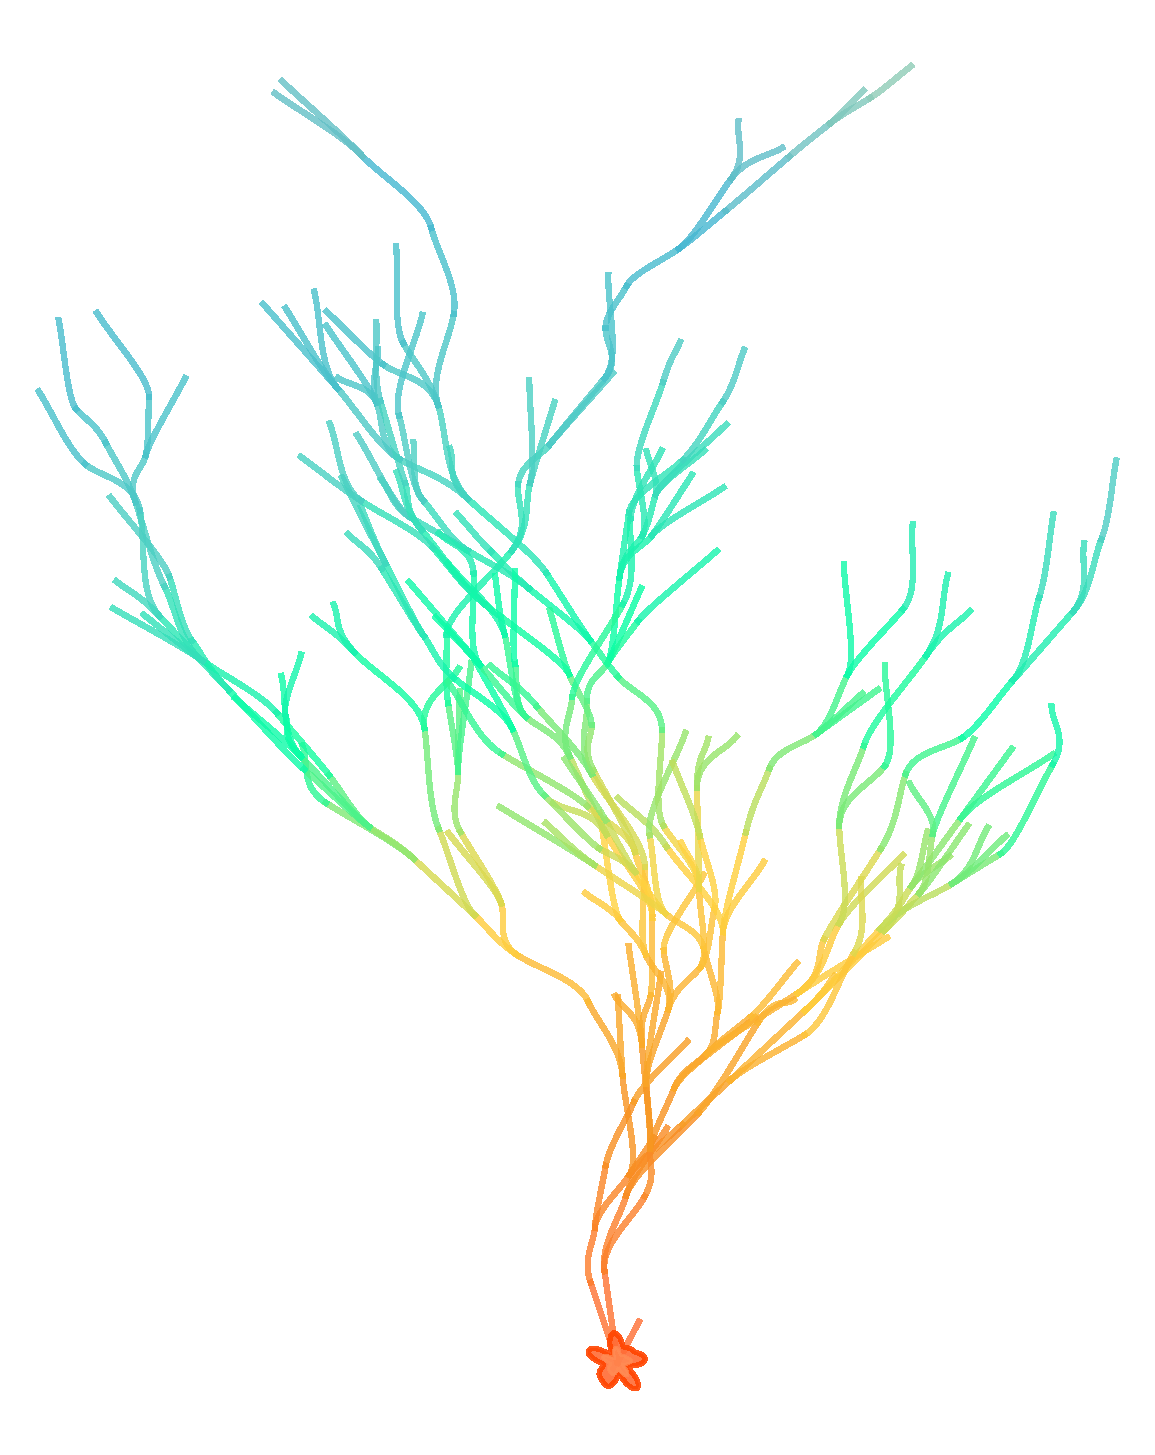
\includegraphics[width=0.25\textwidth]{assets/neuron_stylized.pdf}
        &
        {\Huge $\approx$}
        &
        \centering\begin{circuitikz}[scale=0.75, transform shape]
            % AC voltage source
            \draw (0,0) to[sV, v=$V_m(t)$] (0,3.5);
            \draw (0,3.5) to[short] (1.5,3.5);
            
            % Capacitor
            \draw (1.5,3.5) to[C, l=$C_m$] (1.5,0);
            
            % Connect to three branches
            \draw (1.5,3.5) to[short] (6.5,3.5);
            \draw (1.5,0) to[short] (6.5,0);
            
            % Sodium channel (Na+)
            \draw (3.2,3.5) to[vR, l=$g_{Na}$, *-] (3.2,2.0);
            \draw (3.2,2.0) to[battery1, l=$E_{Na}$] (3.2,0.5);
            \draw (3.2,0.5) to[short, -*] (3.2,0);
            
            % Potassium channel (K+)
            \draw (4.8,3.5) to[vR, l=$g_K$, *-] (4.8,2.0);
            \draw (4.8,2.0) to[battery1, l=$E_K$] (4.8,0.5);
            \draw (4.8,0.5) to[short, -*] (4.8,0);
            
            % Leak channel (Cl-)
            \draw (6.5,3.5) to[vR, l=$g_L$, *-] (6.5,2.0);
            \draw (6.5,2.0) to[battery1, l=$E_L$] (6.5,0.5);
            \draw (6.5,0.5) to[short, -*] (6.5,0);
            
            % Ground symbols
            \draw (0,0) node[ground]{};
            \draw (4.8,0) node[ground]{};
        \end{circuitikz}
    \end{tabular}
    \caption{Biological neuron and its Hodgkin-Huxley 
    equivalent circuit representation.}
    \label{fig:neuron_to_circuit}
\end{figure}

The corresponding differential equation describing the membrane potential dynamics is:
\begin{equation}
    C_m \frac{dV_m}{dt} = I_{ext} - g_{Na}(V_m - E_{Na}) - g_K(V_m - E_K) - g_L(V_m - E_L)
\end{equation}
where $I_{ext}$ is the external input current, and each conductance $g_i$ is voltage and time dependent, governed by additional gating variables.

However, as previously mentioned, natural system are often complex, as in this case we have a four dimensional non-linear coupled system, accurate modeling can be computationally infeasible, thus often simplified models are
preferred for large scale simulations, such as the Izhikevich neuron model \cite{1257420} that captures essential spiking dynamics with only two state variables.
\subsection{Discretization} \todo{quanto in dettaglio?}    

\clearpage

\section{Overview of Machine Learning}
Machine Learning (ML) is a subfield of Artificial Intelligence (AI) that focuses on statistical methods and algorithms capable to \textit{learn} from past experiences.
First we need a rigorous definition of what means to learn; \textcite[]{mitchell1997machine} defines it as : "A computer program is said to \textbf{learn} from experience $\mathbf{E}$ with respect to 
some class of tasks $\mathbf{T}$ and performance measure $\mathbf{P}$, if its performance at tasks in $\mathbf{T}$, as measured by $\mathbf{P}$, improves with experience $\mathbf{E}$."

ML can tackle a much wider range of tasks that are difficult to solve with explicit rules based programming, in a certain sense it bypasses
some level of abstraction, we're not learning the task $T$ directly, but we're sampling from the $E$ space, \textbf{examples} which are 
collection of \textbf{features} that are qualitative or quantitative properties of the data that are exploited by the model to learn the task $T$.%\newline
\subsection{The learning problem}
%Let's start with a definition
A formal definition of a machine learning model is given below:
\begin{comment}

\begin{definition}\todo{questo non è comunque abbastanza generico, perchè definisce solo supervised}
Given a I.I.D. unknown probability joint distribution $P(\mathbf{x}, y)$, with $D_{\text{train}} \sim P(\mathbf{x}, y)$, such that $\mathcal{D_{\text{train}}} = \{(\mathbf{x}_i, y_i)\}_{i=1}^{N} \in \mathcal{X} \times \mathcal{Y}$, where 
${\mathbf{x}_i} \in \mathbb{R}^d$ are the input features and ${y_i} \in \mathbb{R}$ (or $\{0,1\}$ for classification) are the target labels, then a \textbf{machine learning model} is a function $f:\mathbb{R}^d \rightarrow \mathbb{R}$ (or $\{0,1\}$) that maps $\mathbf{x}$ to $y$.
    The goal is to find the optimal parameters $\Theta^*$ of the model $f(\mathbf{x}; \Theta^*)$ that minimize a loss function $\mathcal{L}(y, f(\mathbf{x}; \Theta^*))$ over $\mathcal{D_{\text{train}}}$. 
    \footnote{This definition captures the \textit{supervised learning} paradigm. 
    More broadly, in \textit{unsupervised learning}, 
    the data consists only of $\{\mathbf{x}_i\}$ and 
    the goal is to learn the underlying structure of the data (e.g., clusters, latent representations,
     or the data distribution itself) by optimizing a task-specific objective function $\mathcal{J}$ 
     without the use of target labels $y$.}
\end{definition}

\end{comment}

\begin{definition}
Let $p_{\text{data}}(\mathbf{x})$ be an independent identically distributed (i.i.d.) unknown probability distribution over the input space $\mathcal{X}$. 
A dataset is a finite sample drawn from this distribution, $\mathcal{D} = \{\mathbf{x}_i\}_{i=1}^{N} \subset
 \mathcal{X}$, where $\mathbf{x}_i \in \mathbb{R}^d$ are data points (or input features).

A \textbf{machine learning model} is a family of prediction functions $f: \mathcal{X} \to \mathcal{Y}$ parameterized by 
$\theta$. The nature of the model and its goal is defined by the learning paradigm:

\begin{itemize}
    \item In the \textbf{supervised} setting, the data is drawn from a joint distribution $p_{\text{data}}(\mathbf{x}, y)$, 
    so $\mathcal{D}_{\text{train}} = \{(\mathbf{x}_i, y_i)\}_{i=1}^{N}$, with targets $y_i \in \mathcal{Y}$. 
    Here, $\mathcal{Y}$ (e.g., $\mathbb{R}$ for regression or $\{0,1\}$ for classification), 
    and the goal is to find parameters $theta^*$ that minimize a loss function $\mathcal{L}(y, f(\mathbf{x}; \theta))$ 
    quantifying the discrepancy between predictions and true labels.

    \item In the \textbf{unsupervised} setting, the data consists only of inputs $\mathbf{x}_i$. 
    The output space $\mathcal{Y}$ is defined by the specific task (e.g., $\mathbb{R}^k$ for dimensionality reduction, 
    a set of clusters for clustering, or $\mathbb{R}^d$ for generative models). The goal is to find parameters $\theta^*$
     that optimize an objective function $\mathcal{J}(f(\mathbf{x}; \theta), \mathcal{D})$,
      which captures desired structural properties of the data, such as reconstruction error, cluster cohesion, or data likelihood.
\end{itemize}

In both cases, the ultimate objective is for the model $f(\mathbf{x}; \theta^*)$ to generalize well to new, unseen data $\mathcal{D}_{\text{test}} \sim P(\mathbf{x})$. 
\end{definition}

The model $f_{\theta}$\footnote{We will use $f_{\theta}$ as shorthand for $f(\mathbf{x}; \theta)$}  is said to belong to a \textbf{hypothesis space} $\mathcal{H}$, 
which is the set of all possible functions the model can represent by varying its parameters $\theta$.
The choice of model architecture (e.g., linear models, neural networks, decision trees) 
defines the hypothesis space. A larger, more expressive $\mathcal{H}$ can represent more complex functions.
The learning algorithm searches within $\mathcal{H}$ to find the hypothesis 
$f^* = f(\cdot; \theta^*)$ that best approximates the true underlying relationship between inputs and outputs.
%\clearpage
\subsection{Learning Paradigms}
Models learn the data distributions in threen main different styles: \todo{c'è ne sono molti altri semisupervised, active learning etc.,}
\begin{enumerate}
    \item \textbf{Supervised Learning}, where the we aim for accurate predictions.
    \item \textbf{Unsupervised Learning}, tries to find a compact description of the data
    \item \textbf{Reinforcement Learning}, where an agent recursively interact with an environment in order to maximize a cumulative reward signal, trought a certain policy: $\pi^*$.
\end{enumerate} 
Understanding learning is crucial to choose the right modeling technique and architecture for a given task.
In order to have a more compact picture of learning let's decompose the more general distribution: $P(\mathbf{X}, Y)$

\begin{comment}
At the core of ML there are two main concepts: One we've seen before, the \textbf{Learning} process, 
which is the process of finding the optimal parameters $\Theta^*$ of the model such that the loss function $\mathcal{L}(y, f(\mathbf{x}; \Theta^*))$ is minimized with respect to training data, then we have \textbf{Generalization}, 
that is the capability to perform well on unseen data, given a certain distribution $P(\mathbf{x}, y)$. We can formalize these concept by examining how the joint distribution can be
decomposed and how this relates to the learning objective.\newline
\end{comment}
\subsubsection{Generative and Discriminative Learning o (bayesian view)}
The joint distribution $P(\mathbf{X}, Y)$ decomposes as: \todo{Vorrei evitare di spiegare bayes, ma come introduco questi concetti?}

\begin{equation}
    % color the marginal, prior, likelihood and posterior with different colors
    P(\mathbf{X}, Y) = \color{blue}{P(Y|\mathbf{X})}\color{red}{P(\mathbf{X})} 
    \color{black}= \color{green}{P(\mathbf{X}|Y)}\color{purple}{P(Y)}\color{black}
\end{equation}
\begin{equation*}
    \text{Joint} = \color{blue} \text{(Posterior)} \color{black} \cdot \color{red} \text{(Marginal)} \color{black} =
     \color{green} \text{(Likelihood)} \color{black} \cdot \color{purple} \text{(Prior)} \color{black}
\end{equation*}

In machine learning, the primary goal is often to predict the label $Y$ for a given datapoint
$\mathbf{X}$, this is represented by the \textit{posterior distribution}. One could also be interested in approximating the unknown distribution itself
to then generate new samples from it, in that case, are needed \textit{likelihood} and the \textit{prior} distributions.
\newline
% troppo didattico...
%By rewriting in terms of posterior distribution we get what is commonly referred as the \textbf{Bayes' Theorem}. \todo{citabayes}  
Bayesian Decision Theory \cite{barberBRML2011} provides a statistical framework for the design of many machine learning algorithms.
The way models parameters are estimated often reflects whether the approach is \textit{Generative} or \textit{Discriminative}.

\footnote{However, this correspondence is not absolute \cite[p.~312, Ch.~13]{barberBRML2011}: logistic regression
 can also be trained by pure MLE, and generative models can incorporate priors and thus be estimated via MAP.}
Discriminative models rely often on conditional distribution, the posterior, and whenever we can incorporate
prior knowledge on the parameters, inference is performed through \textbf{Maximum A Posteriori} (MAP) estimation \ref{eq:map}, which seek the best
hypotesis ($\theta$) given the data and prior knowledge.\newline


\todo{forse è meglio ridurre il numero di formule e tenerlo più discorsivo?}
\begin{equation}\label{eq:map}
\theta_{\text{MAP}}^* = \arg\max_{\theta} P(\theta|\mathcal{D}) = \arg\max_{\theta} P(\mathcal{D}|\theta)P(\theta)
\end{equation}

On the other hand generative models learn the joint distribution, and are typically trained by a \textbf{Maximum Likelihood Estimation} (MLE) \ref{eq:mle},
fitting the parameters that maximize the likelihood of the data.\newline
%questo era vecchio magari lo posso risusare se devo cambiare qualcosa
%%To do inference, we seek the best hypotesis a model can provide, which means finding the most probable parameters $\theta$ given the data, that's called Maximum A Posteriori (MAP) estimation:
\begin{equation}\label{eq:mle}
\theta_{\text{MLE}}^* = \arg\max_{\theta} P(\mathcal{D}|\theta)
|\theta)
\end{equation}

\subsection{Risk, Generalization and Overfitting o (Empirical view)}
%FOOTNOTE BARBER 13.3 CHAPTER PAGE 314
While the Bayesian perspective \footnote{As said in \cite[p.~314, Ch.~13]{barberBRML2011}, 
Bayesian approach appears to be formally optimal, but a pragmatic approach is possible, 
it can be conditioned by a penalty $\lambda$ on the complexity of the model} provides a probabilistic view for learning,
in practice what is often adopted is called the \textit{empirical} approach based on risk minimization
\cite{Vapnik1998}. This complements it by focusing on measuring and optimizing performance through the loss function,
with the main goal of achieving \textit{generalization}.
We seek a function $f_{\theta}$ that minimizes the expected risk $\mathcal{R}(f_\theta)$ over $p_{\text{data}}(\mathbf{x}, y)$.
The loss function acts as a proxy for the learning process, risk have a dual nature: the expected risk and the empirical risk.

The \textbf{expected risk} (or population risk) of a hypothesis $f_\theta$ measures its 
average performance over the true data distribution.
%
%\begin{equation}
%    \mathcal{R}(f_\theta) = \mathbb{E}_{(\mathbf{x}, y) \sim p_{\text{data}}}[\mathcal{L}(y, f(\mathbf{x}; \theta))]
%\end{equation}
However, we do not have access to the entire $p_{\text{data}}$ we can only observe a finite sample 
$\mathcal{D}_{\text{train}}$, therefore, we approximate 
the expected risk with the \textbf{empirical risk}: $\hat{\mathcal{R}}(f_\theta)$, which
is the average loss over the training set.\newline
%\begin{equation}
%    \hat{\mathcal{R}}(f_\theta) = \frac{1}{N}\sum_{i=1}^{N} \mathcal{L}(y_i, f(\mathbf{x}_i; \theta))
%\end{equation}
The learning problem becomes finding $\theta^*$ that minimizes $\hat{\mathcal{R}}(f_\theta)$ 
over the training set. This is the \textbf{Empirical Risk Minimization} (ERM) principle, 
which forms the foundation of most practical machine learning algorithms.
%The complete risk is thus divded into:
%\begin{equation}
    %% add also Optimization error
%   \mathcal{R}(f_\theta) = \underbrace{\hat{\mathcal{R}}(f_\theta)}_{\text{Empirical Risk}} + \underbrace{(\mathcal{R}(f_\theta) - \hat{\mathcal{R}}(f_\theta))}_{\text{Generalization Gap}}
%\end{equation}
%% Error is important we can decompose the expected error by Statistical Learning Theory

\subsubsection{Risk Decomposition}

%We choose $f_{\theta}$ from $\mathcal{H}$  such that the expected risk can be decomposed as:
Most of the times the space of possible solution is unfanthomably large, thus we need to decompose the risk in order to understand if 
we are generalizing correctly.\newline
Let $f_{\mathcal{H}}^* = \arg\min_{f \in \mathcal{H}} \mathcal{R}(f)$ be the best possible function within the hypothesis space, 
and let $\hat f_{\mathcal{H}} = \arg\min_{f \in \mathcal{H}} \hat{\mathcal{R}}(f)$ denote the empirical risk minimizer found by the learning algorithm.
Then, the population risk of the learned model can be decomposed in: \cite{10.5555/3360093}\cite{Vapnik1998}\cite{mjt_dlt}\cite[pag. 33, Ch 2]{bach2024learning}
%\cite{mjt_dlt}\cite[pag. 33 Ch 2]{bach2024learning}
%\cite[pag. 168, Ch 12.3]{books/daglib/0033642}

%The \textbf{approximation term} reflects the intrinsic limitations of the hypothesis space~$\mathcal{H}$, 
%the \textbf{generalization term} measures the difference between empirical and true performance, 
%and the \textbf{optimization term} accounts for the gap due to imperfect minimization of the empirical risk.

\begin{equation}
    \mathcal{R}(f_\theta) = 
    \underbrace{\mathcal{R}(f_\theta) - \hat{\mathcal{R}}(f_\theta)}_{\text{Generalization error}}
     + \underbrace{\hat{\mathcal{R}}(f_\theta) - \hat{\mathcal{R}}({f^*}_\mathcal{H})}_{\text{Optimization error}} 
     + \underbrace{\hat{\mathcal{R}}(\hat{f}_\mathcal{H}) - \mathcal{R}(f_\mathcal{H}^*)}_{\text{Estimation error}} + \underbrace{\mathcal{R}(f_\mathcal{H}^*)}_{\text{Approximation error}} 
\end{equation}

The approximation error is irreducible because the data-generating process includes 
an intrinsic noise~$\varepsilon$ that cannot be captured by any hypothesis
 in~$\mathcal{H}$. Consequently, learning algorithms must focus on reducing the remaining
  components. When the selected hypothesis~$f_\theta$ is insufficiently 
  expressive, \textbf{underfitting} occurs: the empirical risk $\hat{\mathcal{R}}(f_\theta)$ may be small,
   yet the estimated hypothesis fails to approximate the target function.\footnote{In the case of limited data availability}
    Conversely, if~$f_\theta$ possesses excessive capacity, the estimator
     can \textit{interpolate} $\mathcal{D}_{train}$, attaining negligible empirical risk, but with a large generalization gap; 
     this phenomenon is called \textbf{overfitting}. 

\subsection{Optimizing and Regularizing}\todo{questa è una parte più pragmatica che spiega come si fa learning e come si gestice la complessità}
We extensively talked about different ways of learning, but yet we haven't discussed on how actually the learning is performed.
Many of the modern ML algorithm are based on \textbf{Gradient-Based Optimization} methods \cite{citaqualcosa}, which iteratively update the model parameters $\theta$ in order to minimize the loss function $\mathcal{L}(y, f(\mathbf{x}; \theta))$.
% what we use for the learning in the work is mainly pseudoinverse, ridge regression since we rely on cover theorem
In this work we will focus on 
\todo{comunque nella tesi non facciamo molto uso di gradient based optimization, forse si può sorvolare sui dettagli o serve comunque come background?}
However learning differs from pure optimization, ML methods optimize indirectly with respect to the population risk.
% continua discorso su ottimizzazione e poi vai direrramente sulla parte successiva
The typical ML objective function minimized is:
\begin{equation}
    \mathcal{L(\theta)} = \mathbb{E}_{(\mathbf{x}, y) \sim \mathcal{D}_{train}}[\mathcal{L}(y, f(\mathbf{x}; \theta))] + \lambda \Omega(\mathbf{w}) 
\end{equation}

The term $\Omega(\mathbf{w})$ is a regularization term that allows to control the complexity of the model, $\lambda$
is an hyperparameter that controls the strength of the regularization.

The most common algorithm is the \textbf{Stochastic Gradient Descent} (SGD) \cite{citaqualcosa}, 
which iteratively updates the parameters $\theta$ in the opposite direction of the gradient of the loss function with respect to the parameters.
Typically we start from a configuration $\theta_0$ and at each iteration $t$ we compute the gradient of the loss function
with respect to the parameters $\nabla_\theta \mathcal{L}(\theta_t)$, then we update the parameters using a learning rate $\eta$ that controls the step size of the update.

The learning rule is written as:

\begin{equation}
    \theta_{t+1} = \theta_t - \eta \nabla_\theta \mathcal{L}(\theta_t)
\end{equation}

\subsubsection{Optimization and Regularization in Reservoir Computing} \todo{questa parte va spostata, metterla qui è troppo presto, oppure introduco reservoir prima}
In reservoir computing, the recurrent connections remains fixed after initialization, 
so learning reduces to estimating the readout parameters. 
Given reservoir states collected in the recurent matrix $\mathbf{W_{rec}} \in \mathbb{R}^{N \times d}$
 and targets $\mathbf{Y} \in \mathbb{R}^{N \times m}$, the readout weights $\mathbf{W_{out}} \in \mathbb{R}^{d \times m}$ are obtained by solving a regularized least-squares problem:

\begin{equation}
    \mathbf{W_{out}} = \arg\min_{\mathbf{W}} ||\mathbf{Y} - \mathbf{W}^T \mathbf{W_{rec}}||_2^2 + \lambda ||\mathbf{W}||_2^2
\end{equation}

The Tikhonov coefficient $\lambda \ge 0$ controls the readout capacity and mitigates overfitting. whenever
$N$ or $d$ is large, iterative solvers such as conjugate gradients approximate the same optimum while retaining the regularization term.

\subsubsection{Model selection and Hyperparameters}

\section{Structured Probabilistic Models (Graphical Models)}\todo{Since RNN are Directed Graphical Models}
Qui l'idea è di andare a parlare dei modelli grafici probabilistici e di come questi siano utili per capire i modelli neurali su sequenze

Structured Probabilistic Models are used to describe a probability distribution using a graph (from graph theory) structure,
which nodes represent random variables and edges represent dependencies between them.

What need to add: Directed and Undirected, inference and learning basics, few famous models (HMM, RBM, CRF Energy-Based Models (EBM),
 why structured models are so useful : Information flow, interpretability, prior knowledge, etc.)

\begin{comment}
% filepath: /home/vincent/UniversityNotes/Thesis/notes/chapters/background.tex
\begin{figure}[H]
    \centering
    \begin{tikzpicture}[
        node distance=1.5cm,
        thick,
        >=stealth,
        scale=0.6,
        transform shape
    ]
    
    % Nodes with simple styles
    \node[star, star points=5, minimum size=8mm, draw=red, fill=red!20] (theta) {$\theta$};
    \node[ellipse, minimum width=25mm, minimum height=12mm, draw=blue, fill=blue!20, right=of theta] (p1) {$p(x,c|\theta)$};
    \node[ellipse, minimum width=25mm, minimum height=12mm, draw=blue, fill=blue!20, right=of p1] (p2) {$p(c|x^*,\theta)$};
    \node[diamond, minimum width=30mm, minimum height=15mm, draw=red, fill=red!20, below=of p2] (loss) {$\langle L(c,c^*)\rangle_{p(c|x^*,\theta)}$};
    \node[star, star points=5, minimum size=8mm, draw=red, fill=red!20, below=of loss] (cstar) {$c^*$};
    
    % Input/output labels
    \node[above=2mm of p1] {$x,c$};
    \node[above=2mm of p2] {$x^*$};
    
    % Simple arrows
    \draw[->] (theta) -- (p1);
    \draw[->] (p1) -- (p2);
    \draw[->] (p2) -- (loss);
    \draw[->] (cstar) -- (loss);
    
    \end{tikzpicture}
    \caption{Probabilistic graphical model representation}
    \label{fig:probabilistic_model}
\end{figure}
\end{comment}


\section{Recurrent Neural Networks and Deep Learning}
yadaydayda

\section{Deep Recurrent Neural Networks}\todo{questa parte va riscritta dopo}
Deep Learning had a great impact on the field of machine learning and artificial intelligence. When we consider a 
deep learning model, we are referring to a model that has multiple layers of neurons. 
The most common type of deep learning model is the Multilayer Perceptron (MLP),
 which consists of multiple layers of fully connected neurons. By adding layers to these models
 we are able to learn representation at different scales, each layer take the pattern from the previous layers and is capable 
 to learn a more complex pattern. 
 In this work, we will focus on
 a set of deep learning models known as Recurrent Neural Networks (RNNs).\cite{ELMAN1990179}\todo[color=green!90]{citations needed}
 RNNs are a type of neural network that is designed to handle sequential data. Depth in these architectures usually referes
 to the number of timestep we unroll the network trough time (or sequence). But we can add depth in more than one way,
 one of those is to stack multiple layers of RNNs on top of each other sequentially. 
 
 \todo{Change this image or make a new one or cite it}
 \begin{figure}[H]
    \centering
    \includegraphics[width=0.9\textwidth]{images/deep_architectures.png}
    \caption{Depths in Neural Network}
    \label{fig:rnn}
\end{figure}

\section{Deep Reservoir Computing}\todo{questo vai nei related works}

Reservoir Computing (RC) is a framework introduced by \todo[color=green!90]{cite}, that is designed to 
simplify the training of Recurrent Neural Networks. 
The main point is that we do not need to train the recurrent connections
 of the network, but only an output layer called the readout.